% Chapter Template

\chapter{Results} % Main chapter title

\label{Chapter4} % Change X to a consecutive number; for referencing this chapter elsewhere, use \ref{ChapterX}

%----------------------------------------------------------------------------------------
%	SECTION 1
%----------------------------------------------------------------------------------------

\section{Parametrizing a distributed task scheduler}
%Para testear hay que tener claro qué variables "barrer"
%Cosas que afectan a la complejidad (tiempo, memoria) del problema: Número de tareas, energía de los satélites, número de satélites, ventana de scheduling,.
%Cosas que afectan al M-B: energía de los satélites y número de tareas: desventaja de un scheduling "secuencializado".
%Cosas que afectan al L-G: Delta! Número de satélites.

In the last section all the details of both Local-Global and market-based distributed task schedulers implementations carried out in this Bachelor Thesis have been detailed. However, to be able to detect the differences in the performance of both algorithms, a benchmark of simulations had to be done.

Nevertheless, whenever is wanted to test an algorithm, its input variables and how these do affect to the time and memory spent in resolving a particular problem must be analysed.

First of all, let us highlight the parameters that affect the general scheduling problem, independent of the particular algorithm chosen to solve it (whether it is the Local-Global or the market-based or any other one):

\begin{itemize}
\item \textbf{Number of tasks. } As the number of tasks to be scheduled increase, the problems complexity increases, as we have the same resources (energy, time...) for more work. In this sense, the problem is more difficult to solve.

\item \textbf{Satellites resources. } For the same number of tasks, if we decrease the resources available at the system, we will have the same problem as in the case of increasing number of tasks.

\item \textbf{Number of satellites. } Even though this supposes having more resources available and hence more possibilities of finding out a solution, the increasing number of satellites causes a bigger distributed system to coordinate, which could lead to an unmanageable system full of resources but unable to schedule any task.

\item \textbf{Scheduling window. } If the scheduling window time is increased, the task allocation problem's complexity could increase, as there are more timing combinations available to \emph{test}. However, if it is set to a very low value, it could create an unsolvable problem, as the same tasks are trying to be nested in an insufficient time period.
\end{itemize}

Secondly, we will enumerate the variables that particularly can influence on the performance of the Local-Global policy:

\begin{itemize}
\item \textbf{Golden index. } This variable is of course completely particular to this algorithm as it is a value defined for it. For very high values of the golden index, more sub-solutions combinations are possible and therefore the complexity of the problem is greater (see \ref{eq_LG_complexity}). This potential dependence is mitigated in part for low values of golden index thanks to the optimizations of the global combinatorial search.

\item \textbf{Number of satellites. } Although this parameter affects the abstract scheduling problem, it's influence on the Local-Global should be highlighted as the number of sub-solutions combinations to be analysed by the \emph{Global} entity depends exponentially of this variable. This influence is also palliated by the global search.
\end{itemize}

Finally, the market-based algorithm variable analysis lead us to highlight the following:

\begin{itemize}
\item \textbf{Satellites resources. } The algorithm results can be quite poor in terms of the optimality if the final schedule when the satellite have not much resources, because this lead to high bid calculations and therefore to large scheduling process times and less scheduled tasks.

\item \textbf{Number of tasks. } The market-based has a big handicap in the ``sequentialization'' that it introduces in the scheduling process: each task is processed and scheduled in non-overlapping rounds, so a high number of tasks could lead to a overloaded system not able to schedule tasks at the same velocity that they arrive in the system.
\end{itemize}

Sweeping these parameters will show us the behaviour of each algorithm and its input limits (i.e. the limits on the input's complexity for the algorithm to be able to solve it in a reasonable period of time and spending a reasonable amount of memory). Moreover, this previous analysis should be confirmed by the experimental simulations shown below.

\section{Performance Tests}

After having theoretically analysed the critical variables for the generic scheduling problem and for each one of the algorithms, experimental simulations have been carried out.

In order to have a good testing platform for being able to perform extensive simulations sweeping the critical variables and executing several tests for a statistically measure, a simple tester application tester has been implemented. This application receives the set of input variables (number of satellites, number of tasks, golden index, scheduling window...) and the sweep required for them. Then it first simulates an Erlang execution with random generated tasks satisfying the input parameters and after that a Local-Global environment, using the same task set for both. Finally, it measures the time and memory expense and reports it to an output file, in such a format that can be easily processed by a specific Matlab script, also developed for this Bachelor Thesis. Each simulation is performed several times for being able to statistically approximate the real behaviour.

Six main test sets have been performed: three tests in which one out of the main critical variables (i.e. number of satellites, number of tasks and golden index) have been fixed while the other two were swept and three tests sweeping only one of the three variables in order to find the limits on the problem size for each algorithm to be able to solve it\footnote{the sweeping ranges and the fixed values are chosen from the most representative cases.}. For a better comprehension and analysis of each one of the simulations performed, the results will be shown in three different sections: first the Local-Global policy and the market-based results are separately analysed, and finally both are compared.

%-----------------------------------
%	SUBSECTION 1
%-----------------------------------
\subsection{Local-Global}

The time spent in solving each problem of the benchmark is shown in figures \ref{fig_tLG_satsfix}, \ref{fig_tLG_tasksfix} and \ref{fig_tLG_goldenfix}. It can be observed that for this values of number of satellites and golden index the time is almost constant, thanks to the optimizations that have been implemented in the \emph{Global} entity, explained in section \ref{sec_LG_optimizations}. However, the number of tasks causes a linear growth in the execution time.

A similar analysis can be done in terms of memory usage: the global combinatorial search optimizations reduce the effects of increasing the number of satellites (the memory used when sweeping this variable is nearly constant) and the golden index (in this case, the memory increases linearly with a small slope). The memory consumption for each test can be see in figures \ref{fig_mLG_satsfix}, \ref{fig_mLG_tasksfix} and \ref{fig_mLG_goldenfix} respectively.

\begin{figure}[ht]
  \begin{minipage}[b]{0.5\linewidth}
    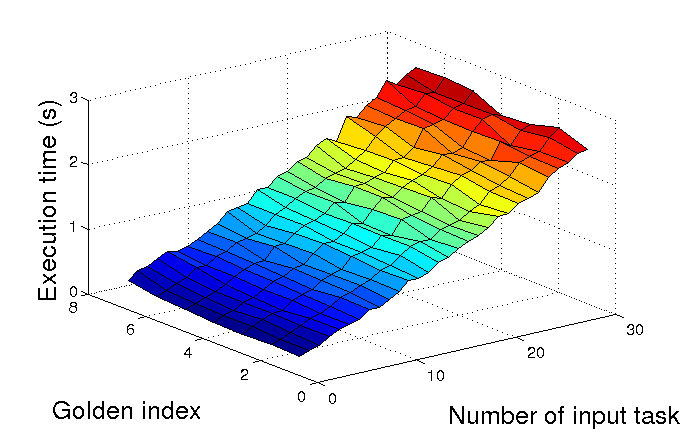
\includegraphics[width=\linewidth]{Figures/tLG_satsfix.png}
    \caption{Execution time (satellites fixed)}\label{fig_tLG_satsfix}
  \end{minipage}  
  \begin{minipage}[b]{0.5\linewidth}
    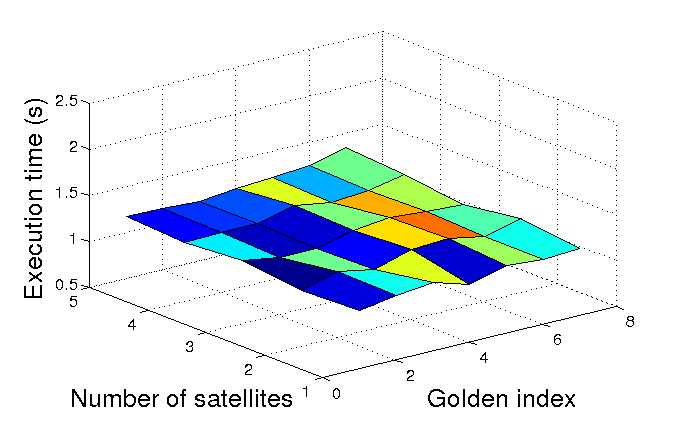
\includegraphics[width=\linewidth]{Figures/tLG_tasksfix.png}
    \caption{Execution time (input tasks fixed)}\label{fig_tLG_tasksfix}
  \end{minipage}  

  \begin{minipage}[b]{0.5\linewidth}
    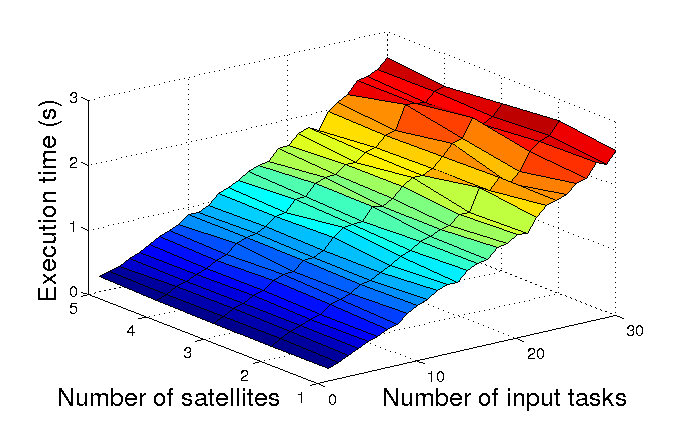
\includegraphics[width=\linewidth]{Figures/tLG_goldenfix.png}
    \caption{Execution time (golden index fixed)}\label{fig_tLG_goldenfix}
  \end{minipage}
    \begin{minipage}[b]{0.5\linewidth}
    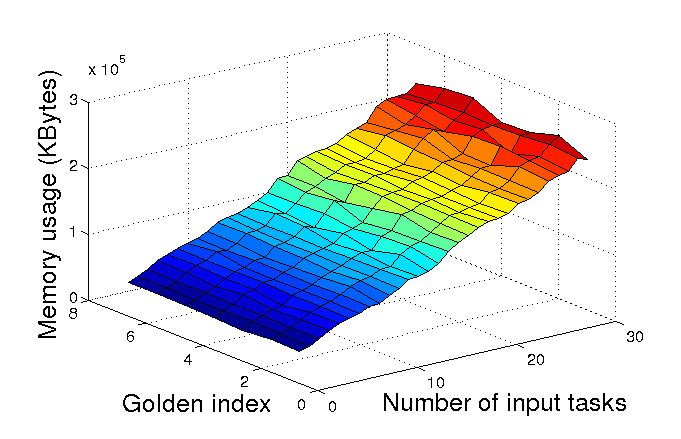
\includegraphics[width=\linewidth]{Figures/mLG_satsfix.png}
    \caption{Memory usage (satellites fixed)}\label{fig_mLG_satsfix}
  \end{minipage}
  
  \begin{minipage}[b]{0.5\linewidth}
    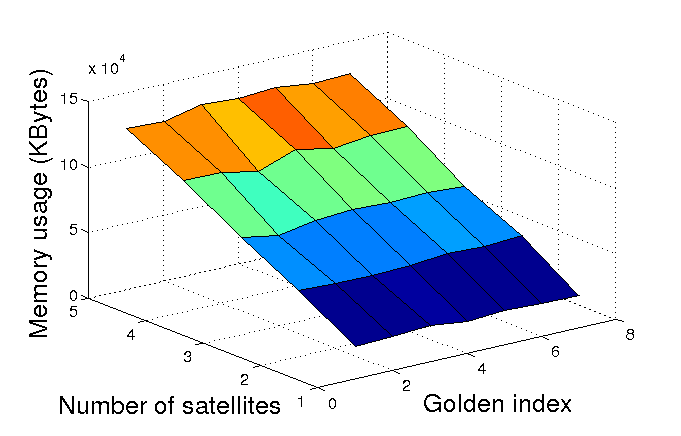
\includegraphics[width=\linewidth]{Figures/mLG_tasksfix.png}
    \caption{Memory usage (input tasks fixed)}\label{fig_mLG_tasksfix}
  \end{minipage}  
  \begin{minipage}[b]{0.5\linewidth}
    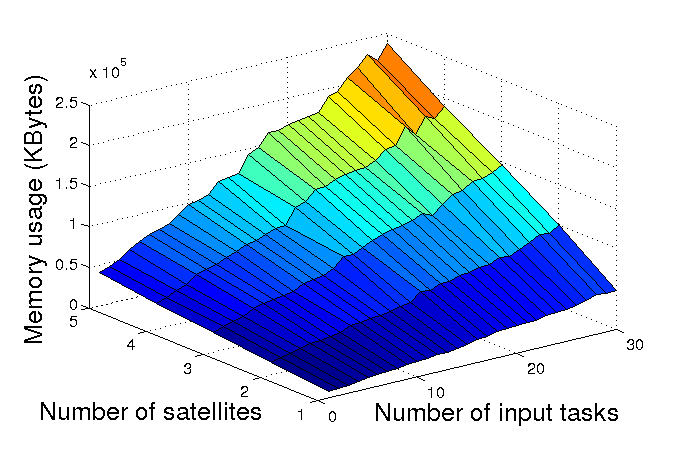
\includegraphics[width=\linewidth]{Figures/mLG_goldenfix.png}
    \caption{Memory usage (golden index fixed)}\label{fig_mLG_goldenfix}
  \end{minipage}
  \hfill
\end{figure}

However, the mitigation achieved for low values of satellites and golden index for time and memory measures is not preserved for high values, as we can observe in figures \ref{fig_tmLG_slim}, \ref{fig_tmLG_alim}, and \ref{fig_tmLG_glim}. Nevertheless, the linear dependence from input tasks is kept.

\begin{figure}[ht]
  \begin{minipage}[b]{\linewidth}
    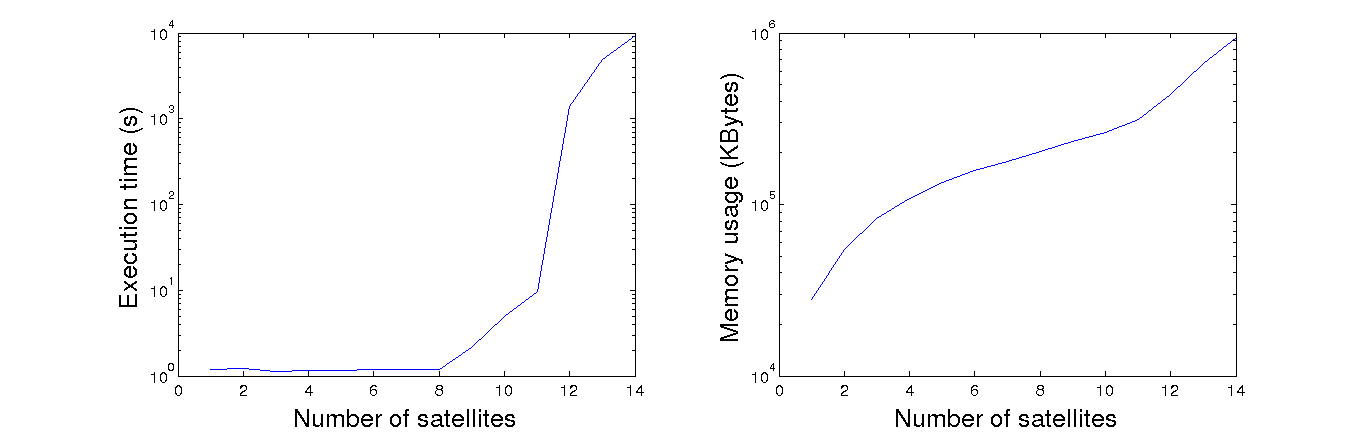
\includegraphics[width=\linewidth]{Figures/tmLG_slim.png}
    \caption{Execution time and memory usage (varying number of satellites)}\label{fig_tmLG_slim}
  \end{minipage}
  
  \begin{minipage}[b]{\linewidth}
    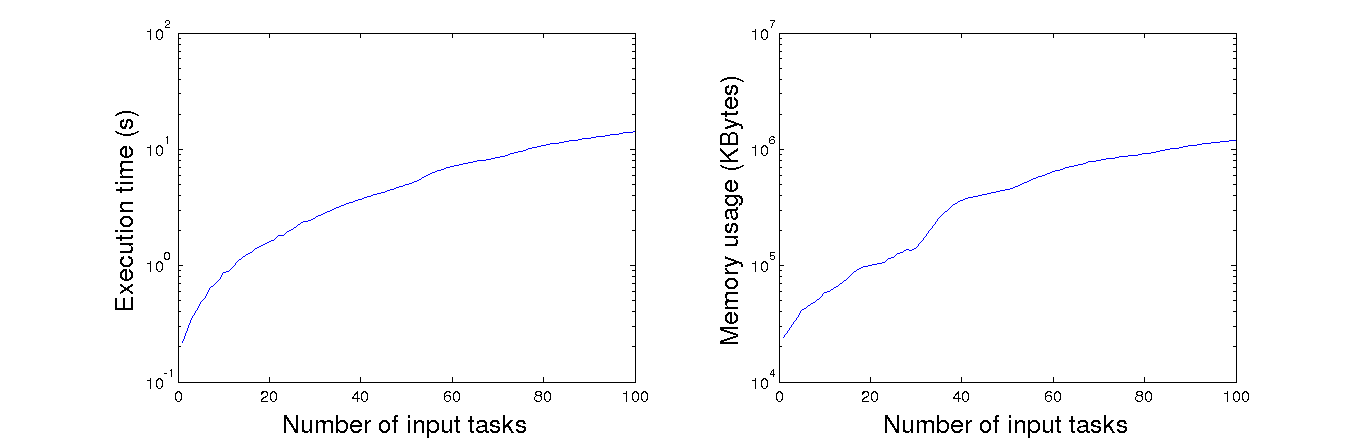
\includegraphics[width=\linewidth]{Figures/tmLG_alim.png}
    \caption{Execution time and memory usage (varying number of input tasks)}\label{fig_tmLG_alim}
  \end{minipage}  

  \begin{minipage}[b]{\linewidth}
    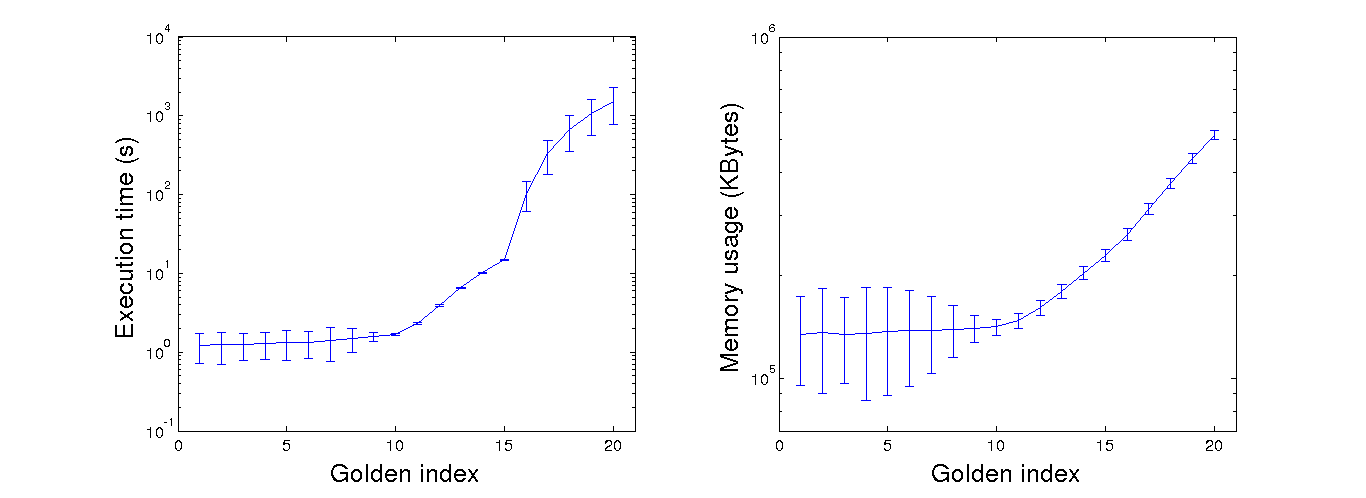
\includegraphics[width=\linewidth]{Figures/tmLG_glim.png}
    \caption{Execution time and memory usage (varying golden index)}\label{fig_tmLG_glim}
  \end{minipage}
  \hfill
\end{figure}

Finally, the total scheduled task number (i.e. the number of tasks that are present in the final schedule solution) is represented in figures \ref{fig_aLG_satsfix} (number of satellites fixed) and \ref{fig_aLG_goldenfix} (golden index fixed). Both plots are very similar and highlight an important characteristic of the behaviour of the Local-Global policy with the implementation carried out in this Bachelor Thesis: for less than 10 input tasks (in this particular benchmark) the system achieves a final schedule which schedules them all. Then, the system begins to saturate and it is not able to schedule all the input tasks. However, the ability of scheduling more tasks at high number of input tasks increases, but not at the same rate than the one of the input tasks. In Fig. \ref{fig_aLG_alim} a final constant saturation point at 80 input tasks can be observed. This behaviour can be optimized by enhancing the \emph{Local} entity so it sends better sub-solutions, as the one implemented for this Thesis still produces some suboptimal sub-solutions that affect the combining capabilities of the \emph{Global}.

\begin{figure}[ht]
  \begin{minipage}[b]{0.5\linewidth}
    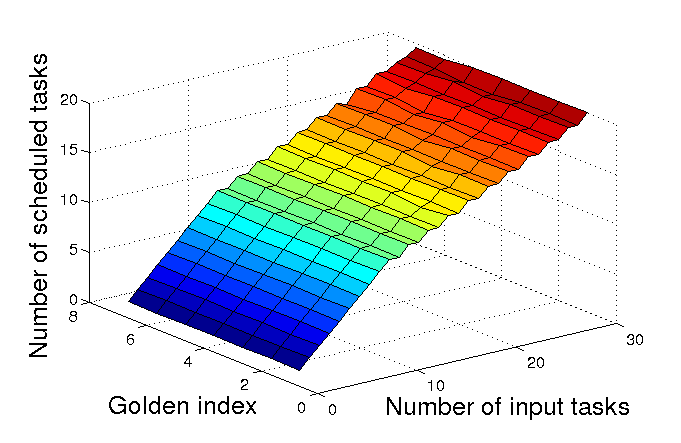
\includegraphics[width=\linewidth]{Figures/aLG_satsfix.png}
    \caption{Execution time (Local-Global)}\label{fig_aLG_satsfix}
  \end{minipage}   
  \begin{minipage}[b]{0.5\linewidth}
    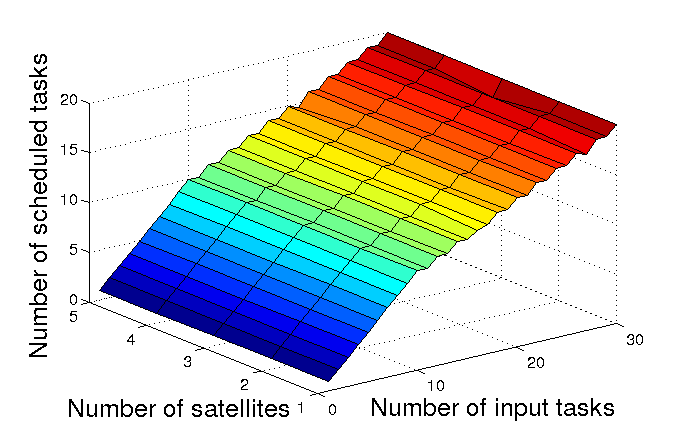
\includegraphics[width=\linewidth]{Figures/aLG_goldenfix.png}
    \caption{Scheduled tasks (Local-Global)}\label{fig_aLG_goldenfix}
  \end{minipage}

  \begin{minipage}[b]{\linewidth}
  \centering
    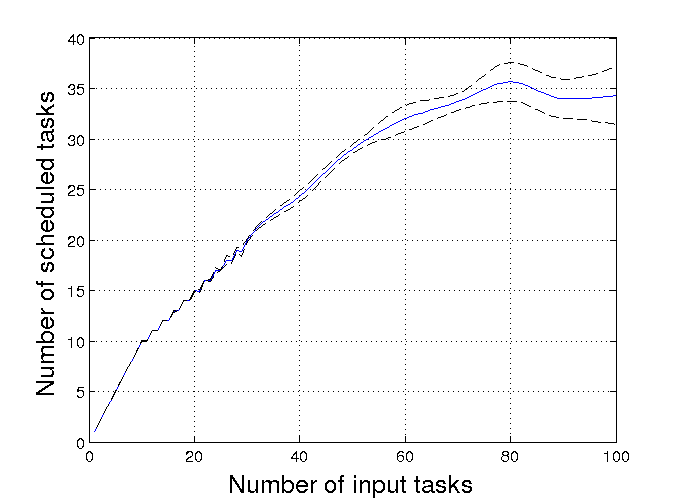
\includegraphics[width=0.6\linewidth]{Figures/aLG_alim.png}
    \caption{Large input tasks range (Local-Global)}\label{fig_aLG_alim}
  \centering
  \end{minipage}
  \hfill
\end{figure}

In this policy, special attention to the global combinatorial search optimizations must be paid. To quickly analyse the improvement it represents to the entire policy, a performance comparison with a brute-force search has been carried out. Results are shown in Fig. \ref{fig_global_brute}, where the mitigation (in the optimized version) of exponential increase with the problem size is clearly observed.

\begin{figure}[ht]
  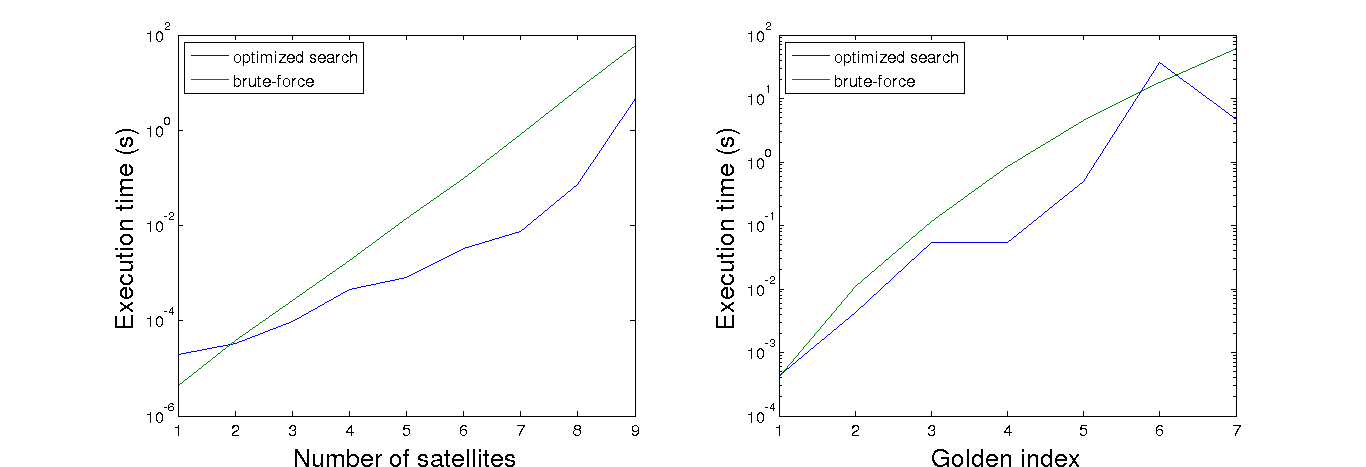
\includegraphics[width=\linewidth]{Figures/global.png}
  \caption{Execution time comparison (combinatorial search vs. brute force)}\label{fig_global_brute}
\end{figure}

%-----------------------------------
%	SUBSECTION 2
%-----------------------------------

\subsection{Price-based}

The price-based results analysis is simpler, as there are only two main variables to sweep: number of satellites and number of tasks. The test results are shown in Fig. \ref{fig_tMB_sw} for time measures, in Fig. \ref{fig_mMB_sw} for memory measures and in Fig. \ref{fig_aMB_sw} for scheduled tasks number.

Regarding time and memory, a clear influence of the increase in the number of tasks is observed, while the number of satellites do not affect the final result. The results in the finally scheduled number of tasks must be highlighted: the price-based algorithm achieves to schedule almost all the input tasks for this values. However, when we sweep over the number of tasks at high values (see Fig. \ref{fig_aMB}), it can be very clearly observed that the performance decreases completely for more than 30 input tasks.

\begin{figure}[ht]
  \begin{minipage}[b]{0.5\linewidth}
    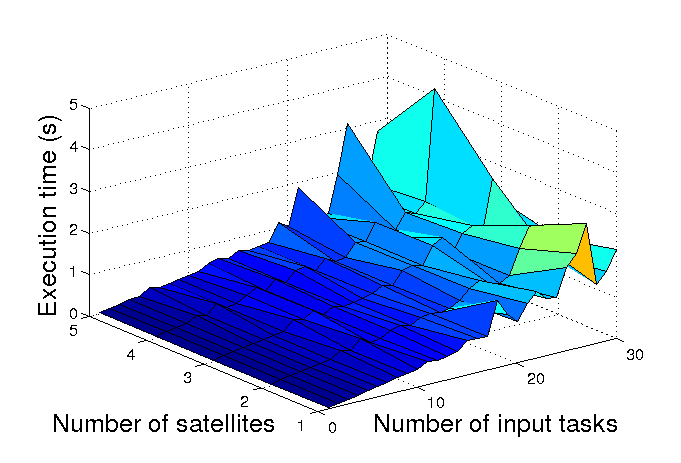
\includegraphics[width=\linewidth]{Figures/tMB_sw.png}
    \caption{Execution time (price-based)}\label{fig_tMB_sw}
  \end{minipage} 
  \begin{minipage}[b]{0.5\linewidth}
    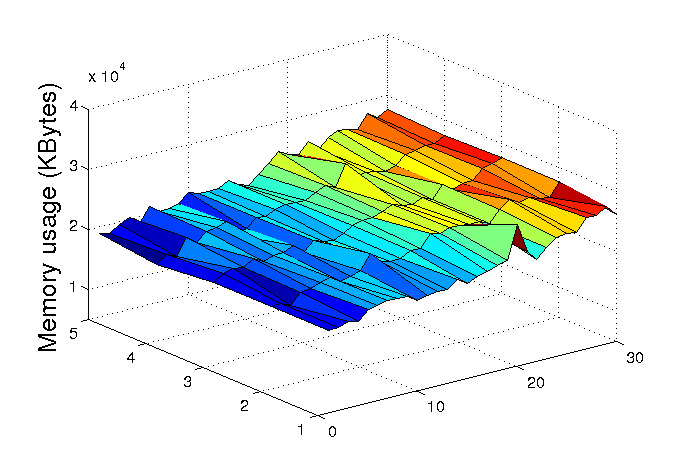
\includegraphics[width=\linewidth]{Figures/mMB_sw.png} 
    \caption{Memory usage (price-based)}\label{fig_mMB_sw}
  \end{minipage} 
  
  \begin{minipage}[b]{0.5\linewidth}
    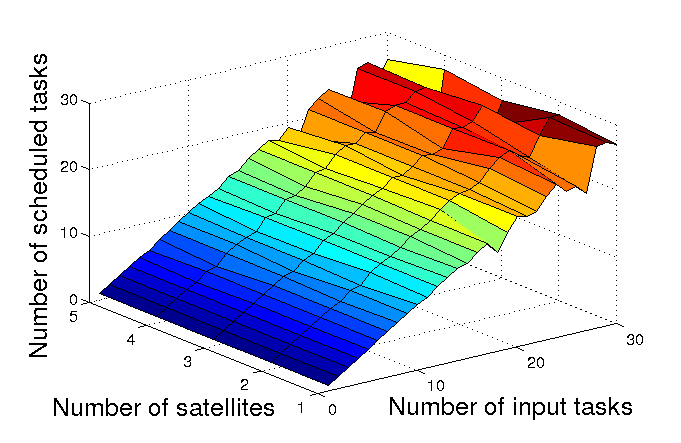
\includegraphics[width=\linewidth]{Figures/aMB_sw.png}
    \caption{Scheduled tasks (price-based)}\label{fig_aMB_sw}
  \end{minipage}
    \begin{minipage}[b]{0.5\linewidth}
    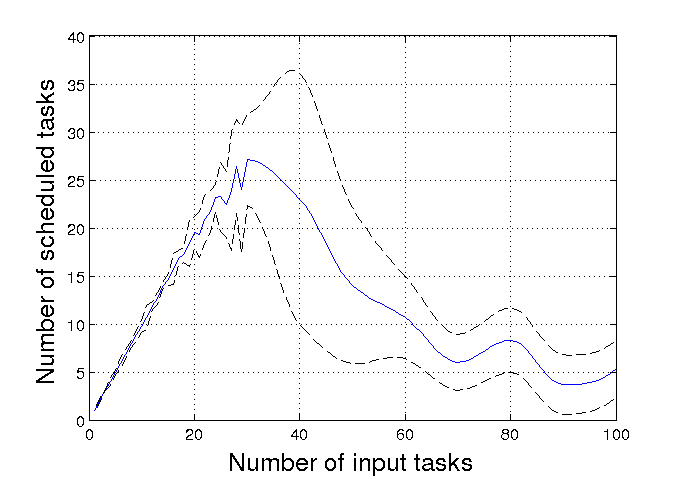
\includegraphics[width=\linewidth]{Figures/aMB.png}
    \caption{Large input tasks range (price-based)}\label{fig_aMB}
  \end{minipage}
  \hfill
\end{figure}

%-----------------------------------
%	SUBSECTION 3
%-----------------------------------

\subsection{The comparison}

As a first concluding result, some comparison representations are shown below, highlighting now the difference in the behaviour of both schedulers that analysing separately each one can remain out of our sight.

Regarding the time spent in solving the input tests, we can observe in Fig. \ref{fig_tLGMB} that both increasing the number of satellites or the number of tasks in the system, the price-based scheduler has lower execution times for almost all the cases. Moreover, the Local-Global policy tends to increase exponentially the resources it spends. The memory utilization behaviour is very similar to the time measures (see Fig. \ref{fig_mLGMB})

However, if we look to the number of scheduled tasks when increasing the number of input tasks (see Fig. \ref{fig_aLGMB}), the Local-Global policy demonstrates its strength on obtaining a near-optimal solution in terms of scheduled tasks (besides other parameters of the solution quality such as satellite utilization or responsiveness): it achieves scheduling more tasks than the price-based scheduler for almost all the tests. The sole range in which the Local-Global is advanced by the price-based is the 10 to 40 range in this case (i.e. between the first saturation point of the Local-Global and the saturation point of the price-based).

\begin{figure}[ht]
  \begin{minipage}[b]{\linewidth}
    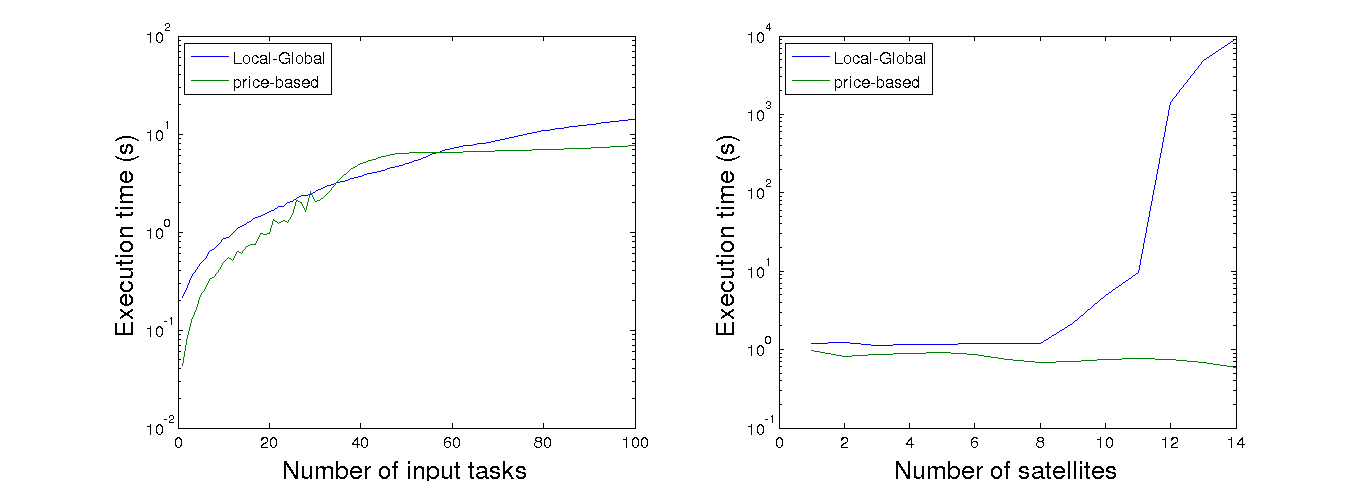
\includegraphics[width=\linewidth]{Figures/tLGMB.png}
    \caption{Execution time comparison}\label{fig_tLGMB}
  \end{minipage} 
  
  \begin{minipage}[b]{\linewidth}
    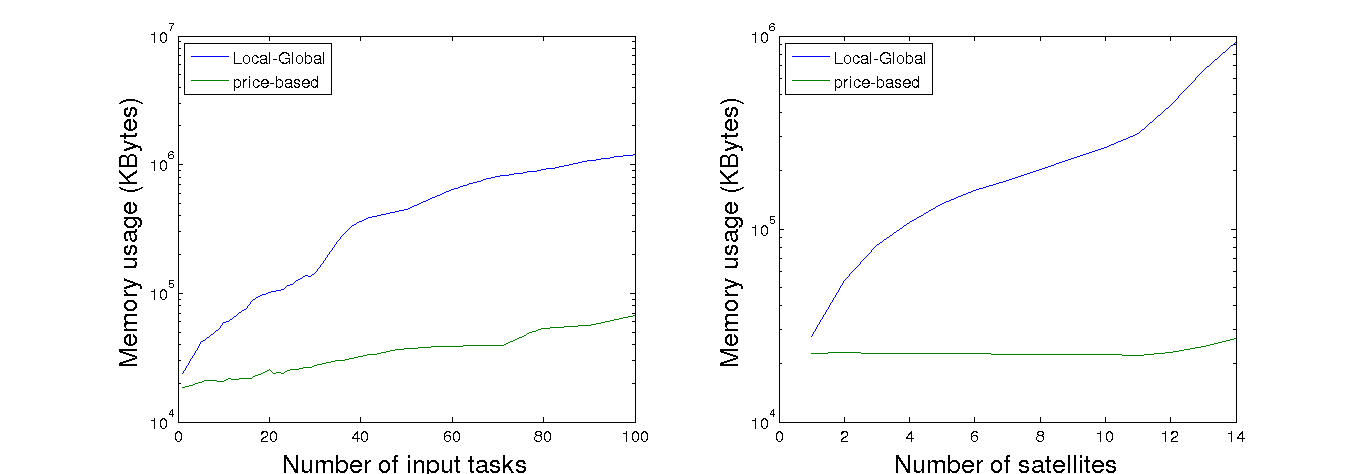
\includegraphics[width=\linewidth]{Figures/mLGMB.png} 
    \caption{Memory usage comparison}\label{fig_mLGMB}
  \end{minipage} 
  
  \begin{minipage}[b]{\linewidth}
  \centering
    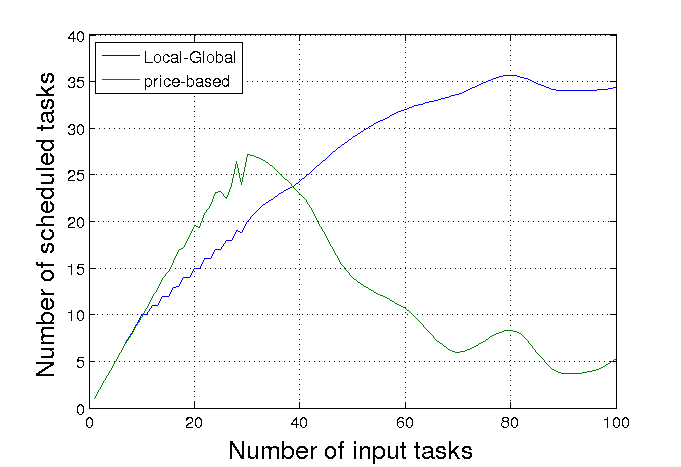
\includegraphics[width=0.6\linewidth]{Figures/aLGMB.png}
    \caption{Scheduled tasks comparison}\label{fig_aLGMB}
  \centering
  \end{minipage}
  \hfill
\end{figure}